\section{Packet Error Rate}

Celem niniejszego podrozdziału jest omówienie przeprowadzonego eksperymentu \gls{PER}. Omówiona zostanie
metodologia badań. Zdefiniowany zostanie termin \textit{pakietu}, który stanowi podstawę dla
doświadczenia.

Wychodząc z definicji, prezentuje się właściwy wzór matematyczny, definiujący badany problem. Równanie
stanowi podstawę dla eksperymentu. Jego zrozumienie pozwoliło zaprojektowanie właściwego doświadczenia
jak i~przygotowanie kompletnego stosu technologicznego niezbędnego do jego przeprowadzenia.

Ostatecznym efektem przeprowadzonego eksperymentu jest przedstawienie zebranych danych pod postacią
wykresów. Prezentują one badane cechy zmienne zaprezentowane w sekcji opisu metodologii. Końcowym
krokiem jest wyciągnięcie wniosków z zebranych danych.
 
%%%%%%%%%%%%%%%%%%%%%%%%%%%%%%%%%%%%%%%%%%%%%%%%%%%%%%%%%%%%%%%%%%%%%%%%%%%%%%%%
%% SUBSECTION: Zależność PER względem odległości między węzłami
%%%%%%%%%%%%%%%%%%%%%%%%%%%%%%%%%%%%%%%%%%%%%%%%%%%%%%%%%%%%%%%%%%%%%%%%%%%%%%%%
\subsection{Metodologia badania}
% poniższe sekcje przerzucić do części teoretycznej
\subsubsection{Definicja pakietu}
Przed przystąpieniem do badań należy precyzyjnie zdefiniować wykorzystywaną terminologię.

Pakietem nazywamy pojedynczą porcję danych przetwarzaną na poziomie warstwy sieciowej modelu ISO OSI \cite{sa_tcpip_nodate}.
Warstwa ta umożliwia routing, adresowanie logiczne oraz przetwarzanie i~dostarczanie pakietów.

\begin{figure}[!ht]
	\centering 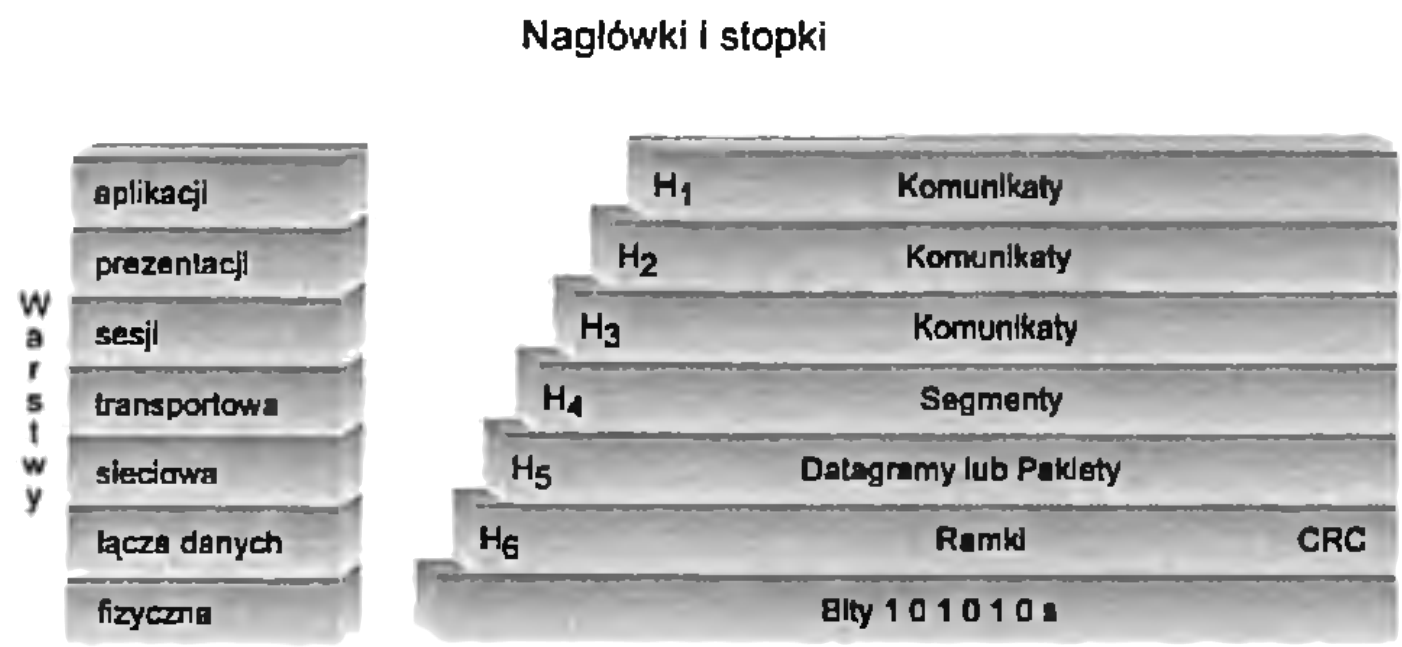
\includegraphics[width=0.618\linewidth]{tcp_ip_szkola_programowania_naglowki_stopki.png} 
	\caption{Model ISO OSI wraz i odpowiadające mu nazwy porcji danych. Źródło: \cite{sa_tcpip_nodate}}
	\label{rys:iso_osi_model_nazwy_grup_danych}
\end{figure}

\gls{BLE} wprowadza własną nomenklaturę dla poszczególnych warstw sieciowych. Jest to o tyle istotne, iż standard ten
nie zapewnia odpowiadających modelowi ISO OSI warstw jeden-do-jednego. Część z tych warstw jest agregowanych w~zespół 
protokołów wyższych warstw - Rysunek~\ref{rys:agregacja_protokolow_ble}. 

Bazując na definicji modelu OSI oraz stosie BLE, pakietem można nazwać wiadomości będące możliwie blisko
warstwy \textit{\gls{LL}}. Podobną definicję prezentuje dokumentacja ST:
\enquote{Pakiet to pojedyncza oznaczona wiadomość wysłana przez jedno i~odebrana przez 
co najmniej jedno urządzenie.}\footnote{Tłumaczenie własne}~\cite{stmicroelectronics_pm0271_2021}

\begin{figure}[!ht]
	\centering 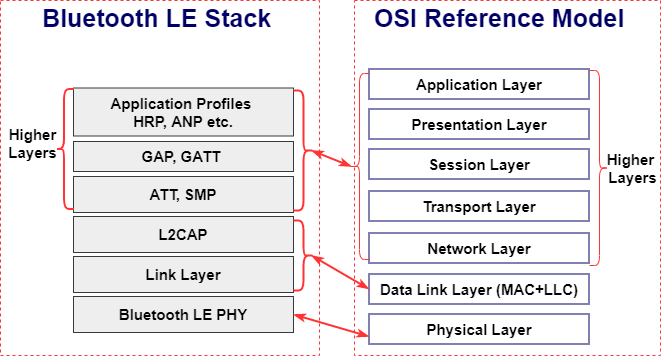
\includegraphics[width=0.618\linewidth]{mathworks_iso_osi_ble_stack.png} 
	\caption{Zestawienie stosu BLE i modelu ISO OSI. Źródło: \cite{noauthor_bluetooth_nodate}}
	\label{rys:agregacja_protokolow_ble}
\end{figure}

BLE Mesh dodatkowo wprowadza własne dodatkowe warstwy komunikacji, biorąc za podstawę stos BLE~\cite{mesh_working_group_mesh_2019}.
Każda z wymienionych warstw jest hermetyzowana za pośrednictwem dostarczanego przez producenta \gls{API}.
Uwzględniając zamknięcie middleware'u i dwu-procesorową architekturę mikrokontrolera STM32WB55, oznacza 
to brak możliwości bezpośredniego nasłuchiwania pakietów w~warstwie \gls{LL}.

Uwzględniając powyższe czynniki, \textit{pakietem} dla BLE Mesh nazywana będzie wiadomość najbliższa warstwie \gls{LL}.
W przypadku stworzonego oprogramowania, oznacza to odbiór komunikatu odebranego jako zdarzenie zarejestrowane przez
koprocesor Cortex-M0, będący integralną częścią mikrokontrolera STM32WB55 odpowiadający za obsługę radia.

\subsubsection{Definicja Packet Error Rate}
Posiadając definicję pakietu, \gls{PER} możliwe staje się zdefiniowanie wzoru, a zarazem znaczenia
głównego celu badań.

PER jest miarą ilości błędnych pakietów w proporcji do wszystkich wysłanych pakietów, zgodnie ze wzorem:

\begin{equation}
\label{per_equation}
PER = \frac{s - r}{s} \cdot 100\%
\end{equation}

gdzie:

\begin{description}
\item[s] is ilość wysłanych pakietów
\item[r] is ilość odebranych pakietów
\item[s-r] - ilość niepoprawnych/błędnych pakietów
\end{description}

Powyższy wzór stanowi podstawę eksperymentu pozwalającego wyznaczyć jakość łącza w zależności od
wybranych parametrów zmiennych.

\subsubsection{Procedura badawcza}\label{subsubsec:test-procedure}

Procedurę badawczą skonstruowano bazując na wzorze~\ref{per_equation}. Niezbędnym mechanizmem, o które oparte
jest doświadczenie, to zliczanie ilości pakietów. Zliczanie dotyczy zarówno węzła bliższego 
jak i~również węzła dalszego odbierającego wysyłane komunikaty. W przypadku drugiego elementu 
opracowano mechanizm odczytywania licznika zmian badanej wartości, patrz: \ref{prep:uc-software}.

Całość doświadczenia przeprowadzono z wykorzystaniem oprogramowania PC - \ref{prep:pc-software}. Oprogramowanie
zapewnia dwie główne funkcjonalności: wysyłanie komunikatów przy określonej częstości przez zadaną ilość czasu;
odczytywanie wartości licznika węzła dalszego.

Wysyłanym komunikatem jest polecenie zmiany stanu modelu
\textit{Generic OnOff}. Wybrano ten standardowy element stosu BLE Mesh ze względu na jego uniwersalność.
Nie ogranicza się on jedynie do wybranej platformy czy własnościowego modelu. Model ten jest zdefiniowany
przez Bluetooth SIG przez co jest niezależny od producenta. Czyni to eksperyment powtarzalny,
niezależnie od mikrokontrolera.

Odczytywanie stanu licznika wymagało wykorzystania autorskiego rozwiązania oparte o własnościowy model Mesh
ST. Nie wpływa to jednak na ostateczny rezultat badań, gdyż stworzone polecenia wykorzystywane jest
tylko do odczytu i~wysłania wartości licznika węzła dalszego do węzła bliższego i~komputera osobistego kontrolującego
przepływ doświadczenia. Z każdą kolejną próbą badania PER ten licznik jest automatycznie zerowany,
przez co sesja zliczeń zawsze rozpoczyna się od zera.

Eksperyment wyznaczający PER oparto o następujące czynniki zmienne:
\begin{itemize}
\item środowisko: teren leśny, teren zurbanizowany
\item interwał zapytań
\item dystans pomiędzy węzłami
\item ilość węzłów składających się na sieć Mesh
\end{itemize}


Wyznaczanie PER odbyło się w dwóch różnych środowiskach. Jednym z głównych hipotez jest znaczący wpływ
środowiska na jakość transmisji danych. Czynniki takie jak temperatura, wilgotność, rodzaj gleby czy
tło radiowe może mieć wpływ na komunikację pomiędzy węzłami. Założono, iż tło radiowe może mieć
największy wpływ ja transmisję danych. Stąd dobrano możliwie skrajne miejsca do badań oceniając
to jako najistotniejszy czynnik:
\begin{itemize}
\item Kampinowski Park Narodowy (lokalizacja: parking Roztoka) - jako teren leśny oddalony od ośrodka miejskiego
ze względnie niewielkim tłem radiowym. Pogoda: pochmurnie, wilgotno, temperatura poniżej 20$^{\circ}$C.
\item Park Pola Mokotowskie - jako teren zurbanizowany charakteryzujący się bogatym tłem radiowym działającym
w pasmach \gls{ISM}. Pogoda: słonecznie, temperatura ok. 20$^{\circ}$C.
\end{itemize}

Kolejnym badanym czynnikiem jest interwał zapytań. Parametr ten został wybrany ze względu na obserwowane
problemy z komunikacją podczas etapu tworzenia oprogramowania. Parametry dobrano w takim stopniu, by ów problem
ukazać. Obrano następujące interwały:
\begin{itemize} \label {items:ping_intervals}
\item 100ms
\item 500ms
\item 800ms
\item 1300ms
\item 2100ms
\end{itemize}

Interesującym parametrem dla bezprzewodowej transmisji danych jest zasięg. Stąd też, jednym z badanych czynników jest
określenie jakości PER w zależności od odległości - Rysunek~\ref{rys:two_nodes_setup}.
\begin{itemize}
\item 1,5m
\item 3,0m
\item 5,0m
\item 8,0m
\item 13,0m
\item 16,0m
\item 21,0m
\end{itemize}

\begin{figure}[!ht]
	\centering 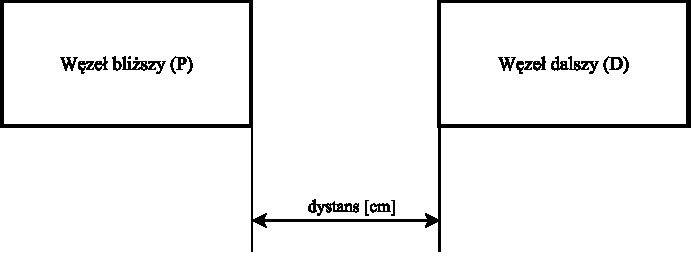
\includegraphics[width=0.618\linewidth]{per_two_nodes.pdf} 
	\caption{Dystans pomiędzy węzłami dla sieci dwóch mikrokontrolerów}
	\label{rys:two_nodes_setup}
\end{figure}

Wyżej wymienione odległości stosowano również w przypadku kolejnego badanego parametru, tj. ilości węzłów
składających się na sieć BLE. W celu łatwej identyfikacji węzłów, wprowadza się następujące nazewnictwo:
\begin{itemize}
	\item węzeł bliższy (ang./łac. \textit{proximal node}/\textit{nodus proximalis}) - węzeł będący połączony bezpośrednio
	ze stacją akwizycji danych i kontroli przepływu eksperymentu.
	\item węzeł środkowy (ang./łac. \textit{intermedial node}/\textit{nodus [inter]medius}) - węzeł działający w trybie
	przekaźnika (terminologia Mesh: \textit{Relay}). Węzeł ten nie uczestniczy bezpośrednio w badaniach tj. nie są
	z niego odczytywane jakiekolwiek dane.
	\item węzeł dalszy (ang./łac. \textit{distal node}/\textit{nodus distalis}) - węzeł zliczający ilość odebranych danych \textit{r},
	udostępniający jednocześnie usługę umożliwiającą odczyt tych wartości tak jak opisano to w podrozdziale \ref{prep:uc-software}.
\end{itemize}

Postanowiono o równoodległym rozstawieniu węzłów - Rysunek~\ref{rys:three_nodes_setup}. Dla sieci 3 węzłów,
maksymalna odległość dzieląca węzeł bliższy od węzła dalszego to 42m. Protokół badawczy zawiera informację 
tylko o odległości w~rozumieniu równoodległego rozstawienia węzłów. Odległość pomiędzy elementami 
jest oczywistą operacją arytmetyczną.

\begin{figure}[!ht]
	\centering 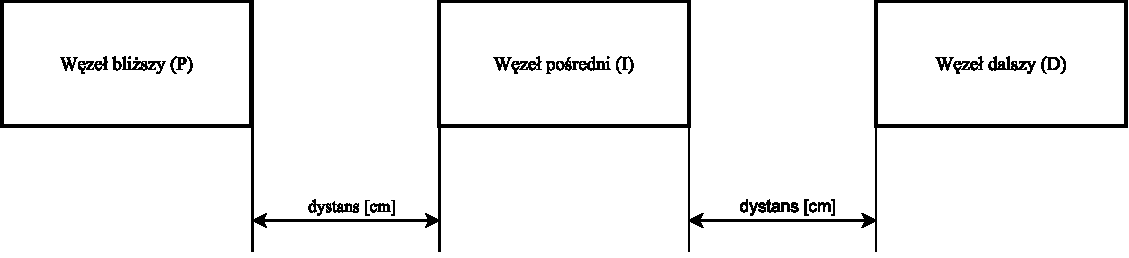
\includegraphics[width=0.99\linewidth]{per_three_nodes.pdf} 
	\caption{Dystans pomiędzy węzłami dla sieci trzech mikrokontrolerów}
	\label{rys:three_nodes_setup}
\end{figure}

Odległość pomiędzy węzłami mierzona jest z użyciem taśmy mierniczej z podziałką 1mm. Tolerancję pomiarów należy
przyjąć jako najdłuższy wymiar zestawu uruchomieniowego P-NUCLEO-WB55 - 70mm \cite{stmicroelectronics_um2435_2019}.
Pomiar odbywał się na płasko, mierząc odległość pomiędzy leżącymi na glebie węzłami. Błędy pomiarowe wynikłe
z ukształtowania terenu są prawdopodobne i~wynikają z~terenowego charakteru badań.

W celu zminimalizowania ryzyka pojawienia się losowych błędów o nieznanym pochodzeniu badanie powtarzano pięciokrotnie,
w sposób następujący: dla wybranego środowiska, ilości węzłów i zadanej odległości pomiędzy węzłami, wykonaj
5 powtórzeń pomiarowych dla każdego z zadanych interwałów pomiarowych.

\begin{equation}
\label{experiment_definition}
\exists e, \exists n, \exists d: PER_i = f(e, n, d), i=1,...,5
\end{equation}

gdzie:

\begin{description}
\item[e] - środowisko
\item[n] - ilość węzłów
\item[d] - równoodległy dystans pomiędzy węzłami
\item[i] - ilość powtórzeń
\item[PER] - Packet Error Rate dla wybranego powtórzenia przy stałych parametrach e, n, d
\end{description}

Wykorzystując tak zebrane dane, wyrysowano je na szeregu wykresów wyznaczając jednocześnie
linie aproksymacyjne z użyciem modelu liniowego wyznaczonego metodą najmniejszych kwadratów. Odchylenia standardowe zaprezentowane
są z użyciem ograniczonego tła otaczającego linię w tym samym kolorze o~zmienionym parametrze nieprzezroczystości.

Parametry transmisji danych nie ulegały zmianie podczas przeprowadzanych doświadczeń. Poniższe wartości należy
przyjąć za stałe:
\begin{itemize}
\item Szybkość transmisji: 2Mbps
\item Moc transmisji danych: 0dBm
\end{itemize}

%%%%%%%%%%%%%%%%%%%%%%%%%%%%%%%%%%%%%%%%%%%%%%%%%%%%%%%%%%%%%%%%%%%%%%%%%%%%%%%%
%% SUBSECTION: Zależność \gls{PER} względem częstości zapytań
%%%%%%%%%%%%%%%%%%%%%%%%%%%%%%%%%%%%%%%%%%%%%%%%%%%%%%%%%%%%%%%%%%%%%%%%%%%%%%%%
\subsection{Zależność PER względem częstości zapytań}

Pierwszą sprawdzaną hipotezą jest empiryczna weryfikacja czy częstość zapytań wpływa na \gls{PER}.
W tym celu wykreślono szereg wykresów dla wybranych interwałów czasowych. Pozostałe parametry traktowane są
jako stałe.

Rysunek~\ref{rys:per_to_distance_under_100ms} przedstawia zależność PER dla interwału 100 milisekund w~zależności
od odległości dla sieci złożonej z dwóch i trzech węzłów. 

\begin{figure}[!htb]
	\centering 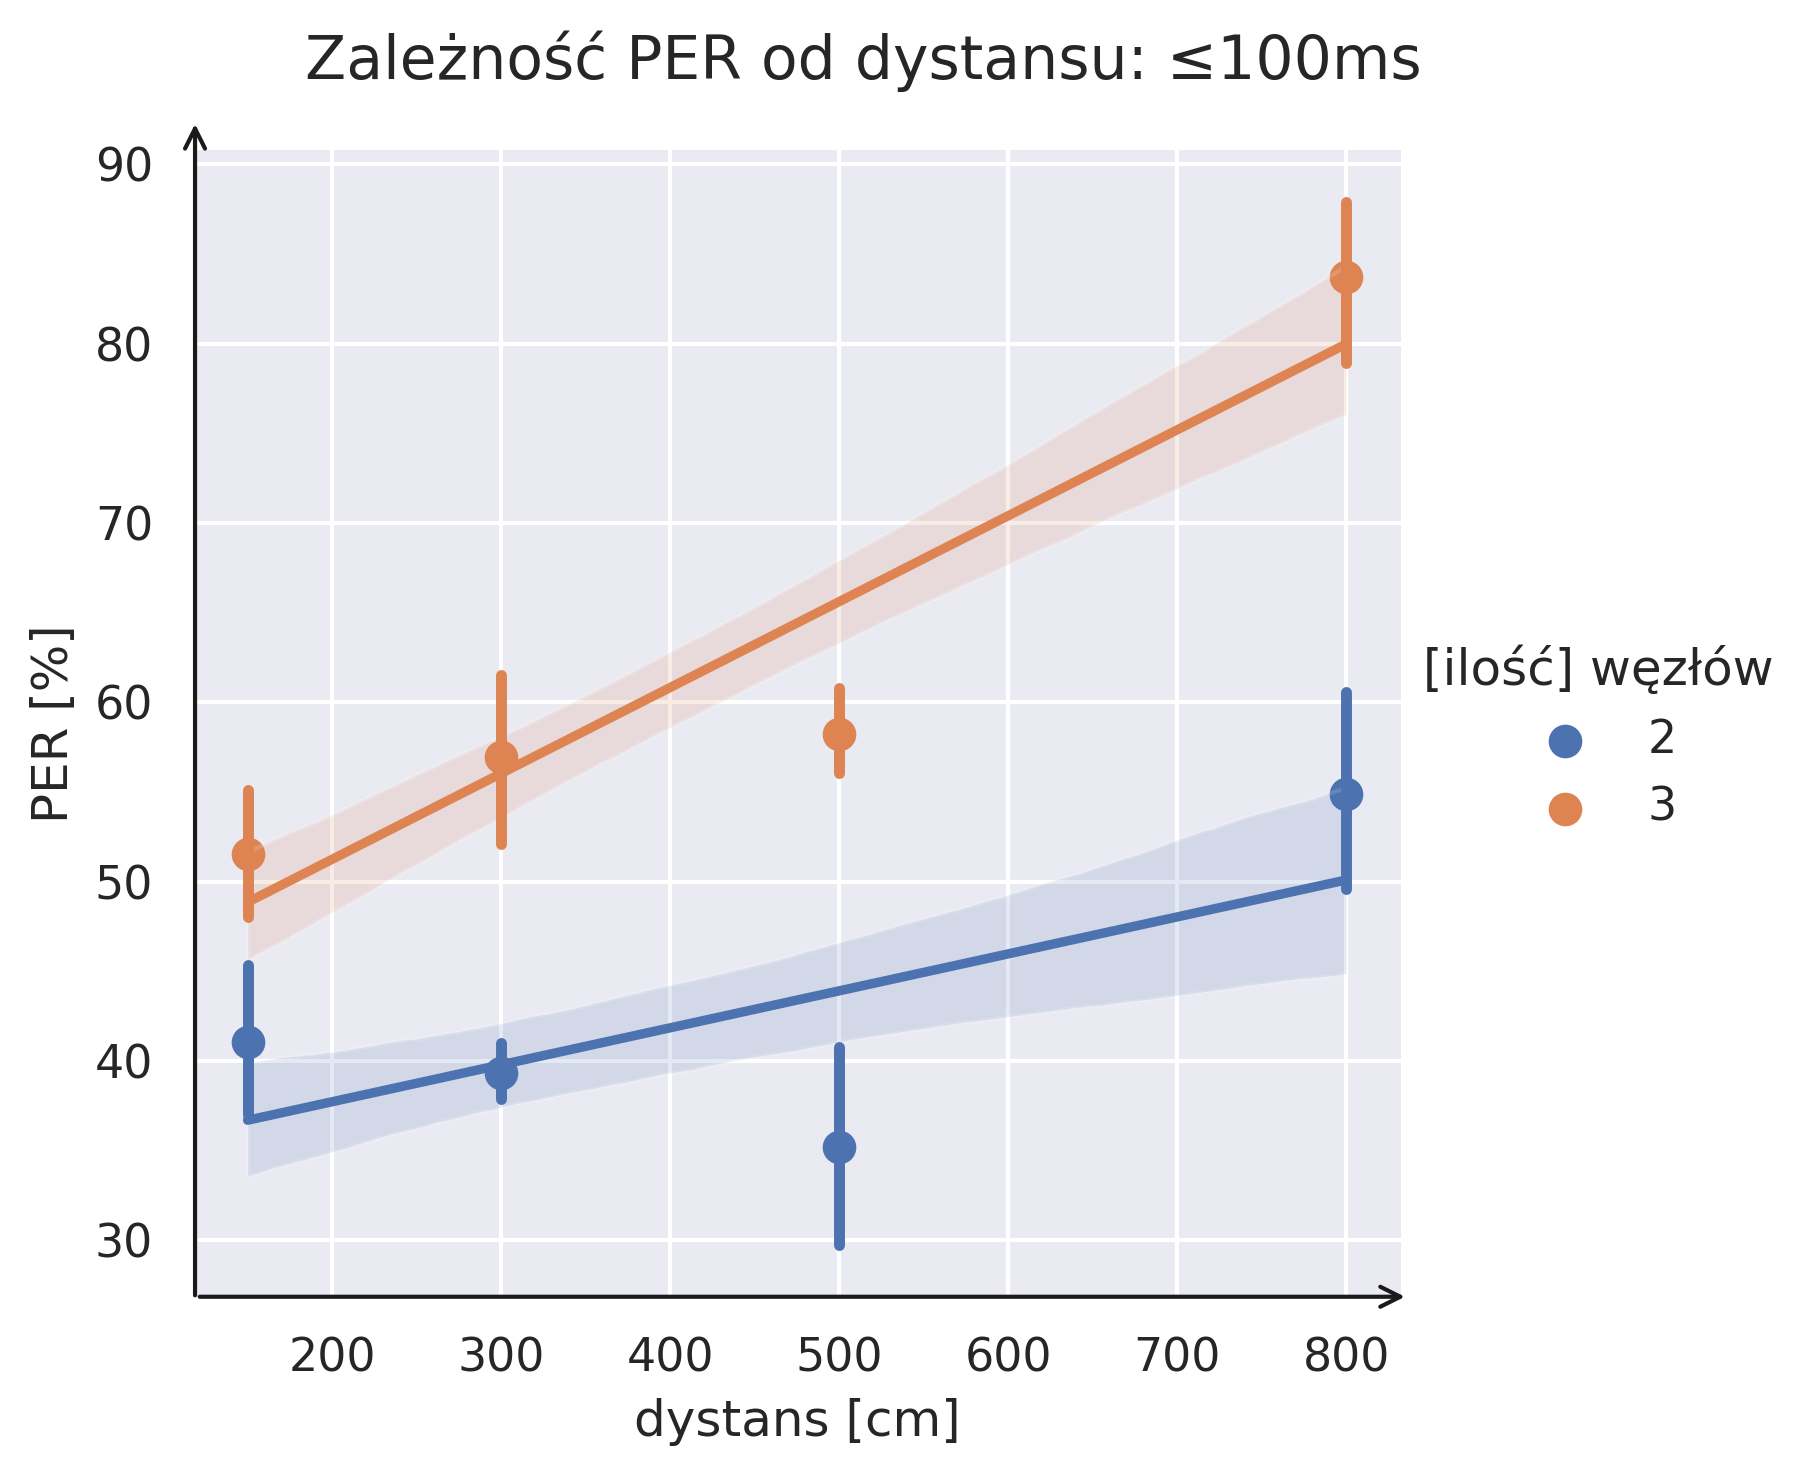
\includegraphics[width=0.618\linewidth]{per_to_distance_under_100ms.png}
	\caption{Zależność \gls{PER} od dystansu dla zapytań o częstości $\leqslant$ 100ms dla różnej liczby węzłów}
	\label{rys:per_to_distance_under_100ms}
\end{figure}

Niewątpliwą cechą ukazanych danych jest wysoka wartość PER już przy tak niewielkiej odległości jak 150 cm pomiędzy węzłami.
Utrata 40-50\% wysyłanych pakietów danych już na pierwszym dystansie pomiarowym może być spowodowana wieloma czynnikami.
Przypuszczalnie, wpływ na taki rezultat wywodzi się z czynników środowiskowych lub ze sposobu wykonywania 
eksperymentu. Niewykluczone są również ograniczenia sprzętowe.

Wraz ze wzrostem odległości pomiędzy węzłami PER wzrasta pomimo wysokiej wartości początkowej. Jest to 
oczekiwana zależność i zgodna z wiedzą techniczną.

Prowadząc dalszą analizę zależności PER od częstości zapytań, sprawdzono wpływ środowiska na jakość transmisji danych.
Rysunek~\ref{rys:per_to_distance_under_100ms_different_envs} przedstawia wybraną zależność. Rozróżnienie
na ilość węzłów nie zostało tutaj uwzględnione. Pomiary przeprowadzone w~najbliższym dobranym dystansie ponownie 
wskazują na 40-50\% utratę pakietów w węźle dalszym. Analogiczne rezultaty obserwowane są na pozostałych dystansach 
z~oczekiwaną tendencją wzrostową.
Wykres dodatkowo przedstawia pewną różnicę w jakości transmisji danych w~zależności od środowiska. Różnica ta 
jednak mieści się w odchyleniu standardowym, posiadając część wspólną dla zadanych parametrów. Nie jest to 
wystarczające do stwierdzenia jednoznacznego wpływu środowiska.

\begin{figure}[!htb]
	\centering 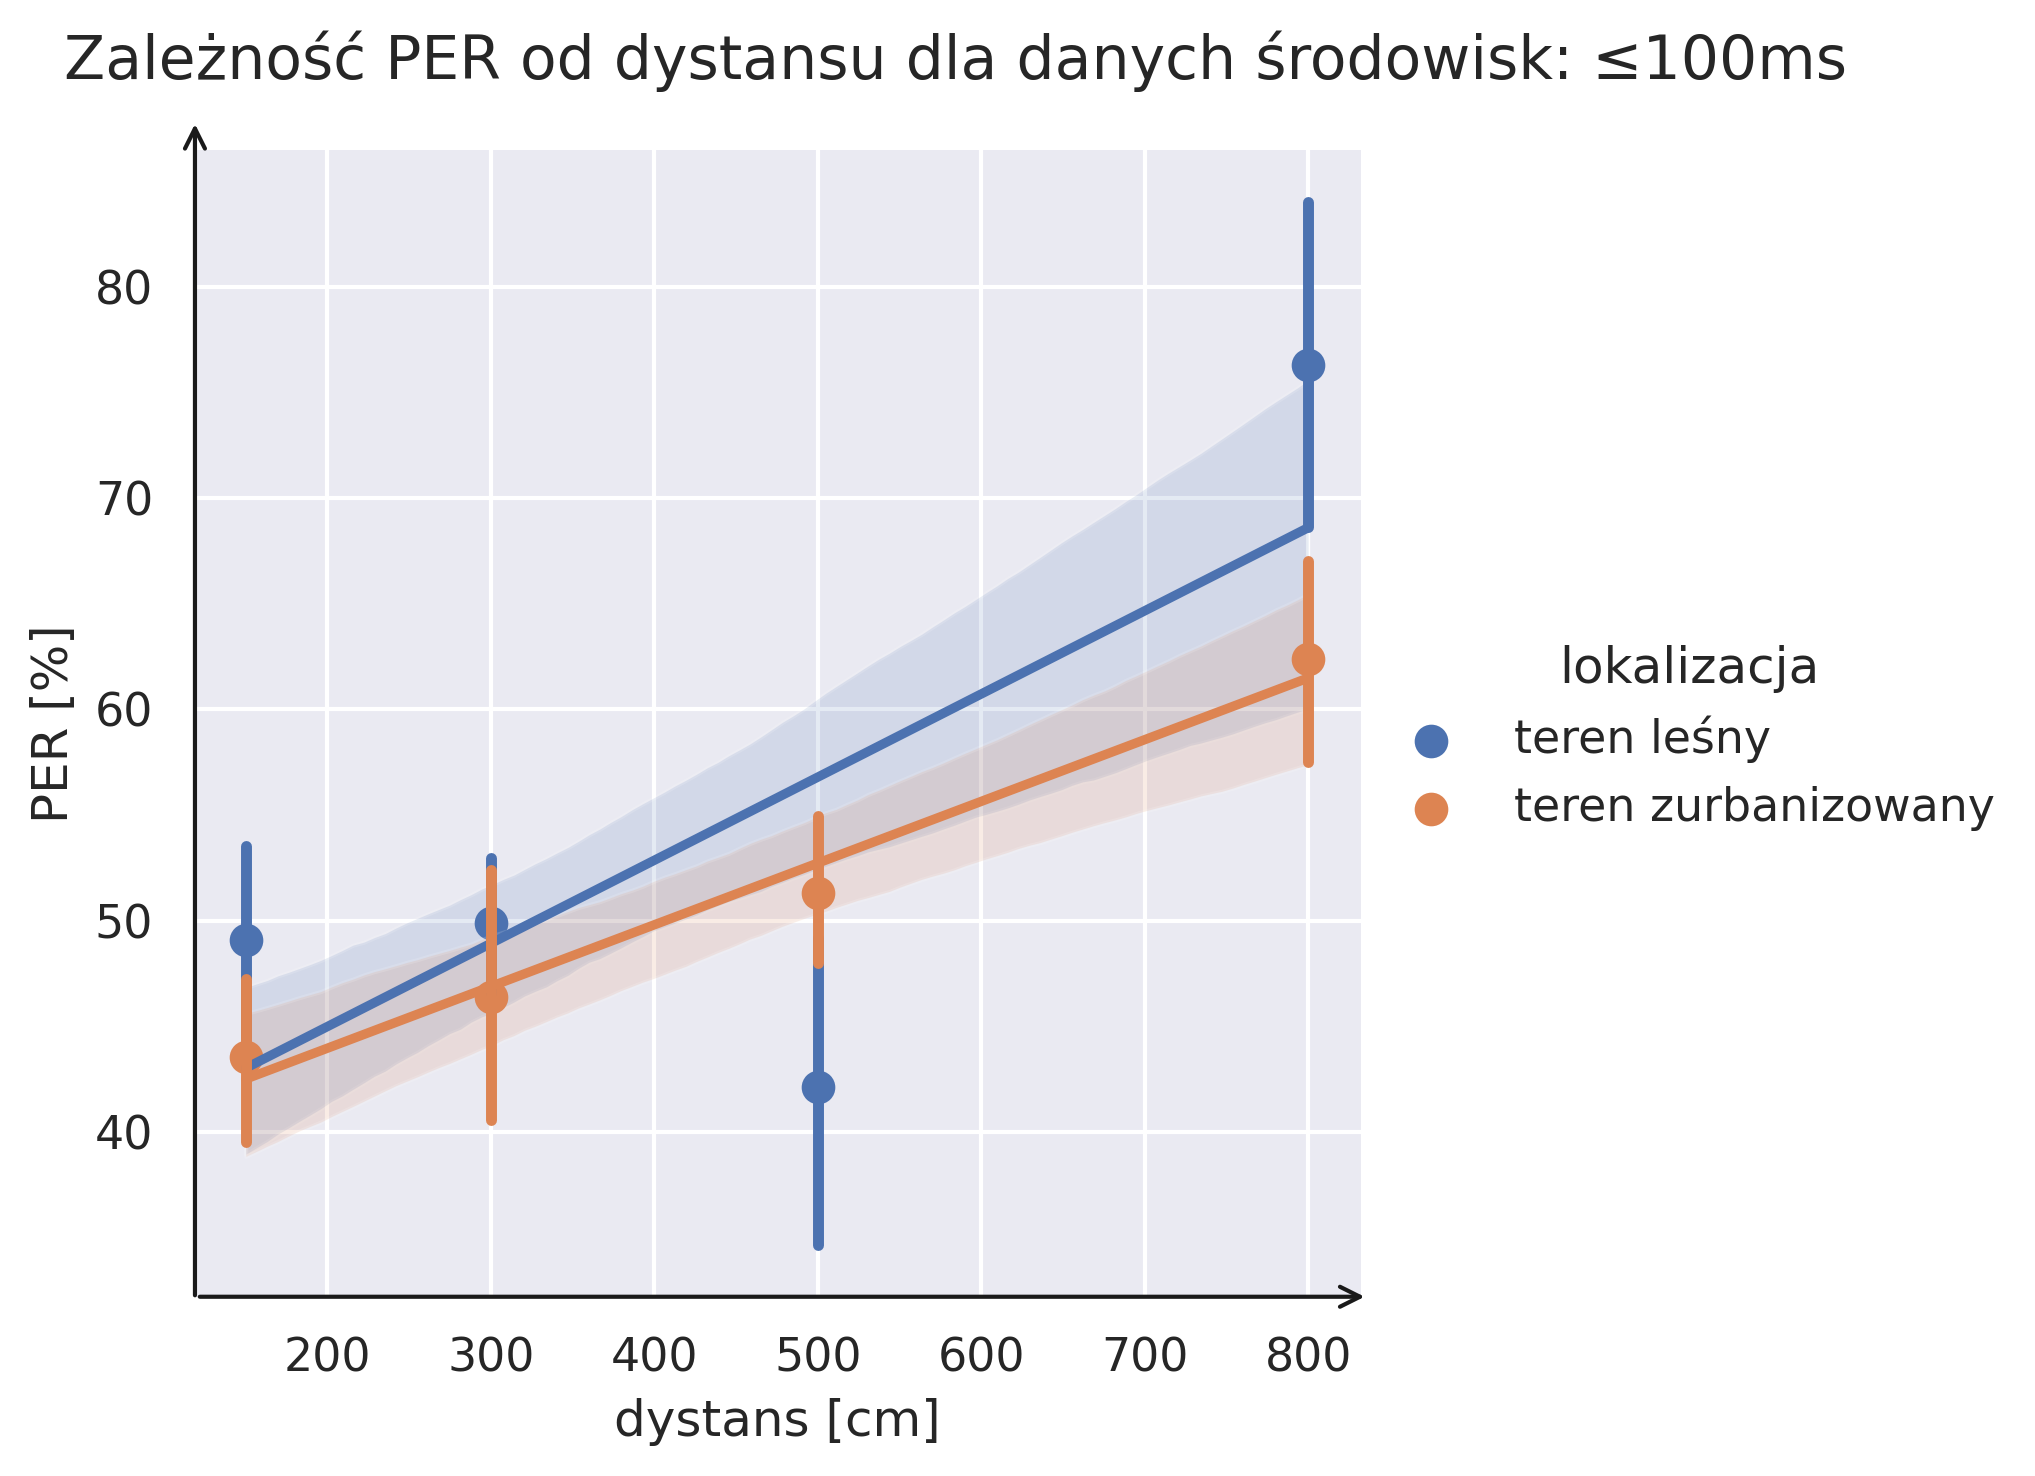
\includegraphics[width=0.618\linewidth]{per_to_distance_under_100ms_different_envs.png} 
	\caption{Zależność \gls{PER} od dystansu dla zapytań o częstości $\leqslant$ 100ms w wybranych środowiskach bez rozróżnienia na liczbę węzłów}
	\label{rys:per_to_distance_under_100ms_different_envs}
\end{figure}

Zestawiając ze sobą wymienione wcześniej czynniki, obserwuje się interesujące zależności. Rysunek~\ref{rys:per_to_distance_under_100ms_different_envs_and_nodes} wskazuje na zależność dystansu, ilości węzłów i rodzaju
środowiska dla wybranego interwału zapytań 100 milisekund. Po raz kolejny obserwowany jest PER wynoszący
40-50\%, niezależnie od środowiska czy ilości węzłów. Sugeruje to wpływ samej testowanej platformy
na ostateczny rezultat. Prawdopodobną hipotezą jest niewystarczająca wielkość zaalokowanych
buforów obsługujących transmisję danych. Mikrokontroler nie będąc w stanie obsłużyć tak częstej transmisji
może doświadczyć awarii, co zaobserwowano podczas badań. Awaria objawiała się brakiem reakcji węzła bliższego
na jakiekolwiek komendy AT, co wymagało ponownego uruchomienia urządzenia. Weryfikacja tego zagadnienia
wymagałaby zaangażowania zaawansowanych narzędzi programistycznych ingerujących m.in. w~pamięć urządzenia.
Niniejsza praca nie podejmuje się wyjaśnienia przyczyn obserwowanych anomalii w działaniu mikrokontrolera,
udostępniając jednocześnie możliwy punkt dla dalszych prac badawczych z zakresu BLE Mesh.

Wpływ samego stosu łączności na PER przy zadanej częstości zapytań zdaje się potwierdzać wykres uwzględniający
jakość transmisji dla dwóch węzłów. Niemalże pozioma linia aproksymacji sugeruje niewielki wpływ dystansu na PER.
Dotyczy to zarówno terenu zurbanizowanego jak i~terenu leśnego. Zbliżone rezultaty zdają się wykluczać
czynniki zewnętrzne.

Interesującą zależnością jest nachylenie wykresu względem osi odciętych. Dla przypadku dwóch węzłów sieci,
połączenie bezpośrednio między węzłami, PER jest niemal stałe na wybranych odległościach, porównywalne
z~przypadkiem terenu leśnego. W przypadku trzech
węzłów, uwidacznia się potencjalny wpływ węzła środkowego, przekazującego pakiety z punktu bliższego do
dalszego. Wraz ze wzrostem dystansu, rośnie wartość PER sięgając nawet 90\% w terenie leśnym. Różne nachylenie
dla wybranych środowisk również sugeruje znaczący wpływ środowiska na PER.

\begin{figure}[!htb]
	\centering 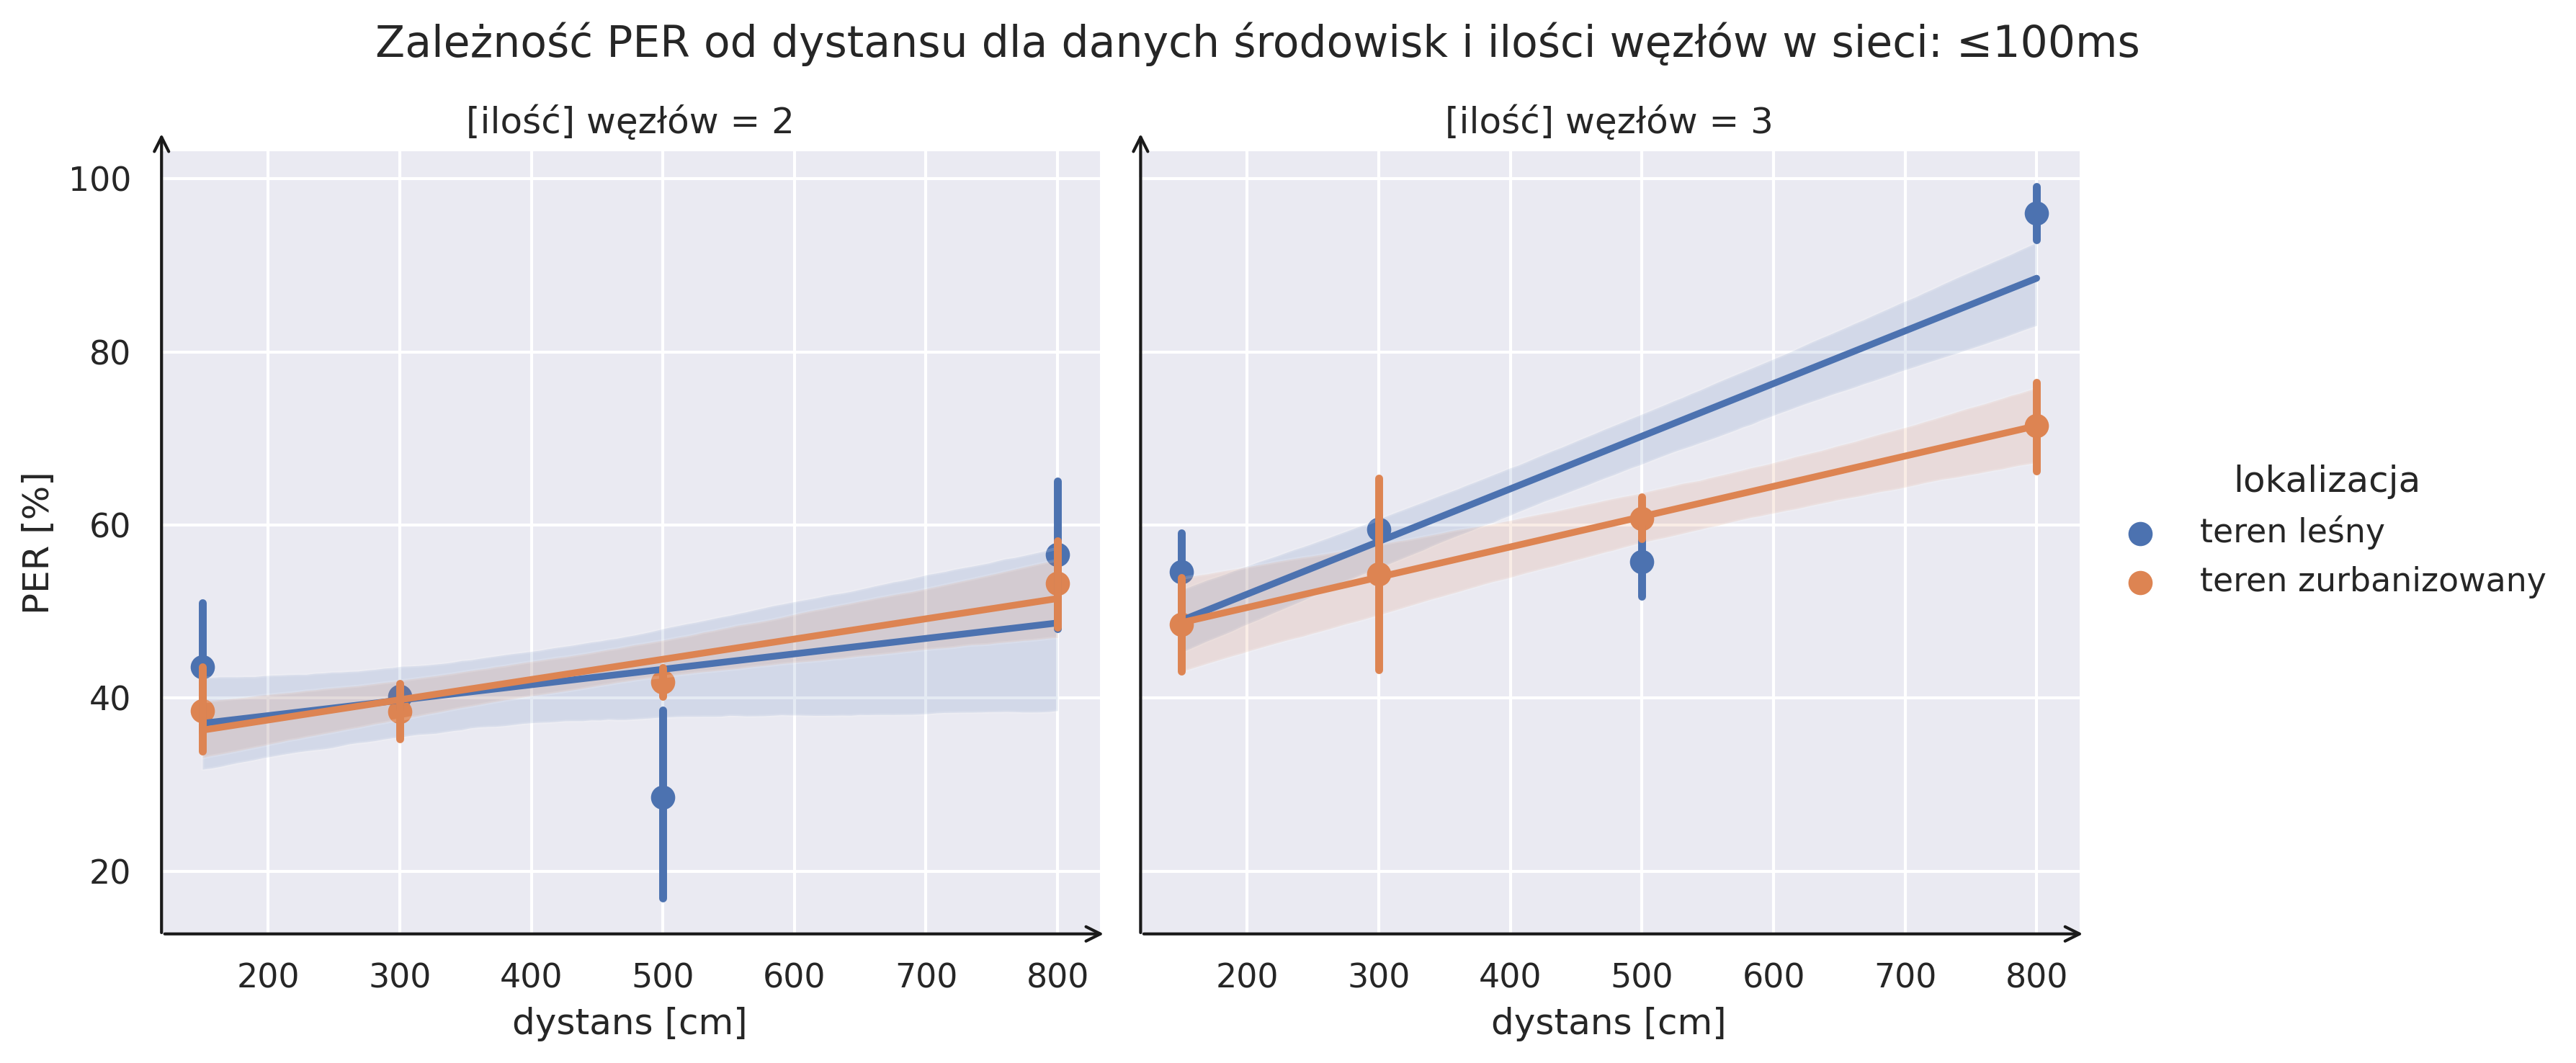
\includegraphics[width=0.99\linewidth]{per_to_distance_under_100ms_different_envs_and_nodes.png}
	\caption{Zależność \gls{PER} od dystansu dla zapytań o częstości $\leqslant$ 100ms w wybranych środowiskach i liczbę badanych węzłów}
	\label{rys:per_to_distance_under_100ms_different_envs_and_nodes}
\end{figure}

Znając charakterystykę łączności dla okresów poniżej 100 milisekund, weryfikuje się pozostałe wybrane częstości, zgodnie
z podanymi wartościami~\ref{items:ping_intervals}. Rysunek~\ref{rys:per_to_distance_over_100ms_different_envs_different_ping_interval}
prezentuje pozostałe interwały w zależności od dystansu i wybranych środowisk bez rozróżnienia na ilość węzłów w sieci.

Przeprowadzone pomiary w terenie leśnym wskazują charakterystykę połączenia zgodną z~intuicyjnymi przewidywaniami.
Na~początkowym dystansie 150cm nie obserwuje się problemów z łącznością. Wszystkie wysłane pakiety zostały
odebrane przez węzeł dalszy. Kolejny dystans wskazuje już na pewną utratę pakietów poniżej 20\%. Prawdopodobnym czynnikiem
jest pogoda lub ukształtowanie terenu leśnego. Co istotne, pomiary dla różnych interwałów odpytywań są zbliżone.
Sugerowałoby to brak wpływu częstości na \gls{PER}. Na pozostałych dystansach pomiarowych, wartości utraty pakietów
są do siebie wzajemnie zbliżone osiągając swoje maksimum na dystansie 21m - blisko 100\% zaginionych pakietów.

Charakterystyka łączności w terenie zurbanizowanym prezentuje się podobnie. Nie obserwuje się znaczącej utraty 
pakietów na względnie bliskich dystansach (150, 300 i 500cm). Wartość PER rośnie wraz ze wzrostem odległości
pomiędzy węzłami osiągając w swoim szczycie wartość ok. 40\%. Co istotne, linie aproksymacyjne są do siebie
zbliżone, ponownie sugerując brak korelacji pomiędzy częstością wysyłania komunikatów a~wartością PER.


\begin{figure}[!htb]
	\centering 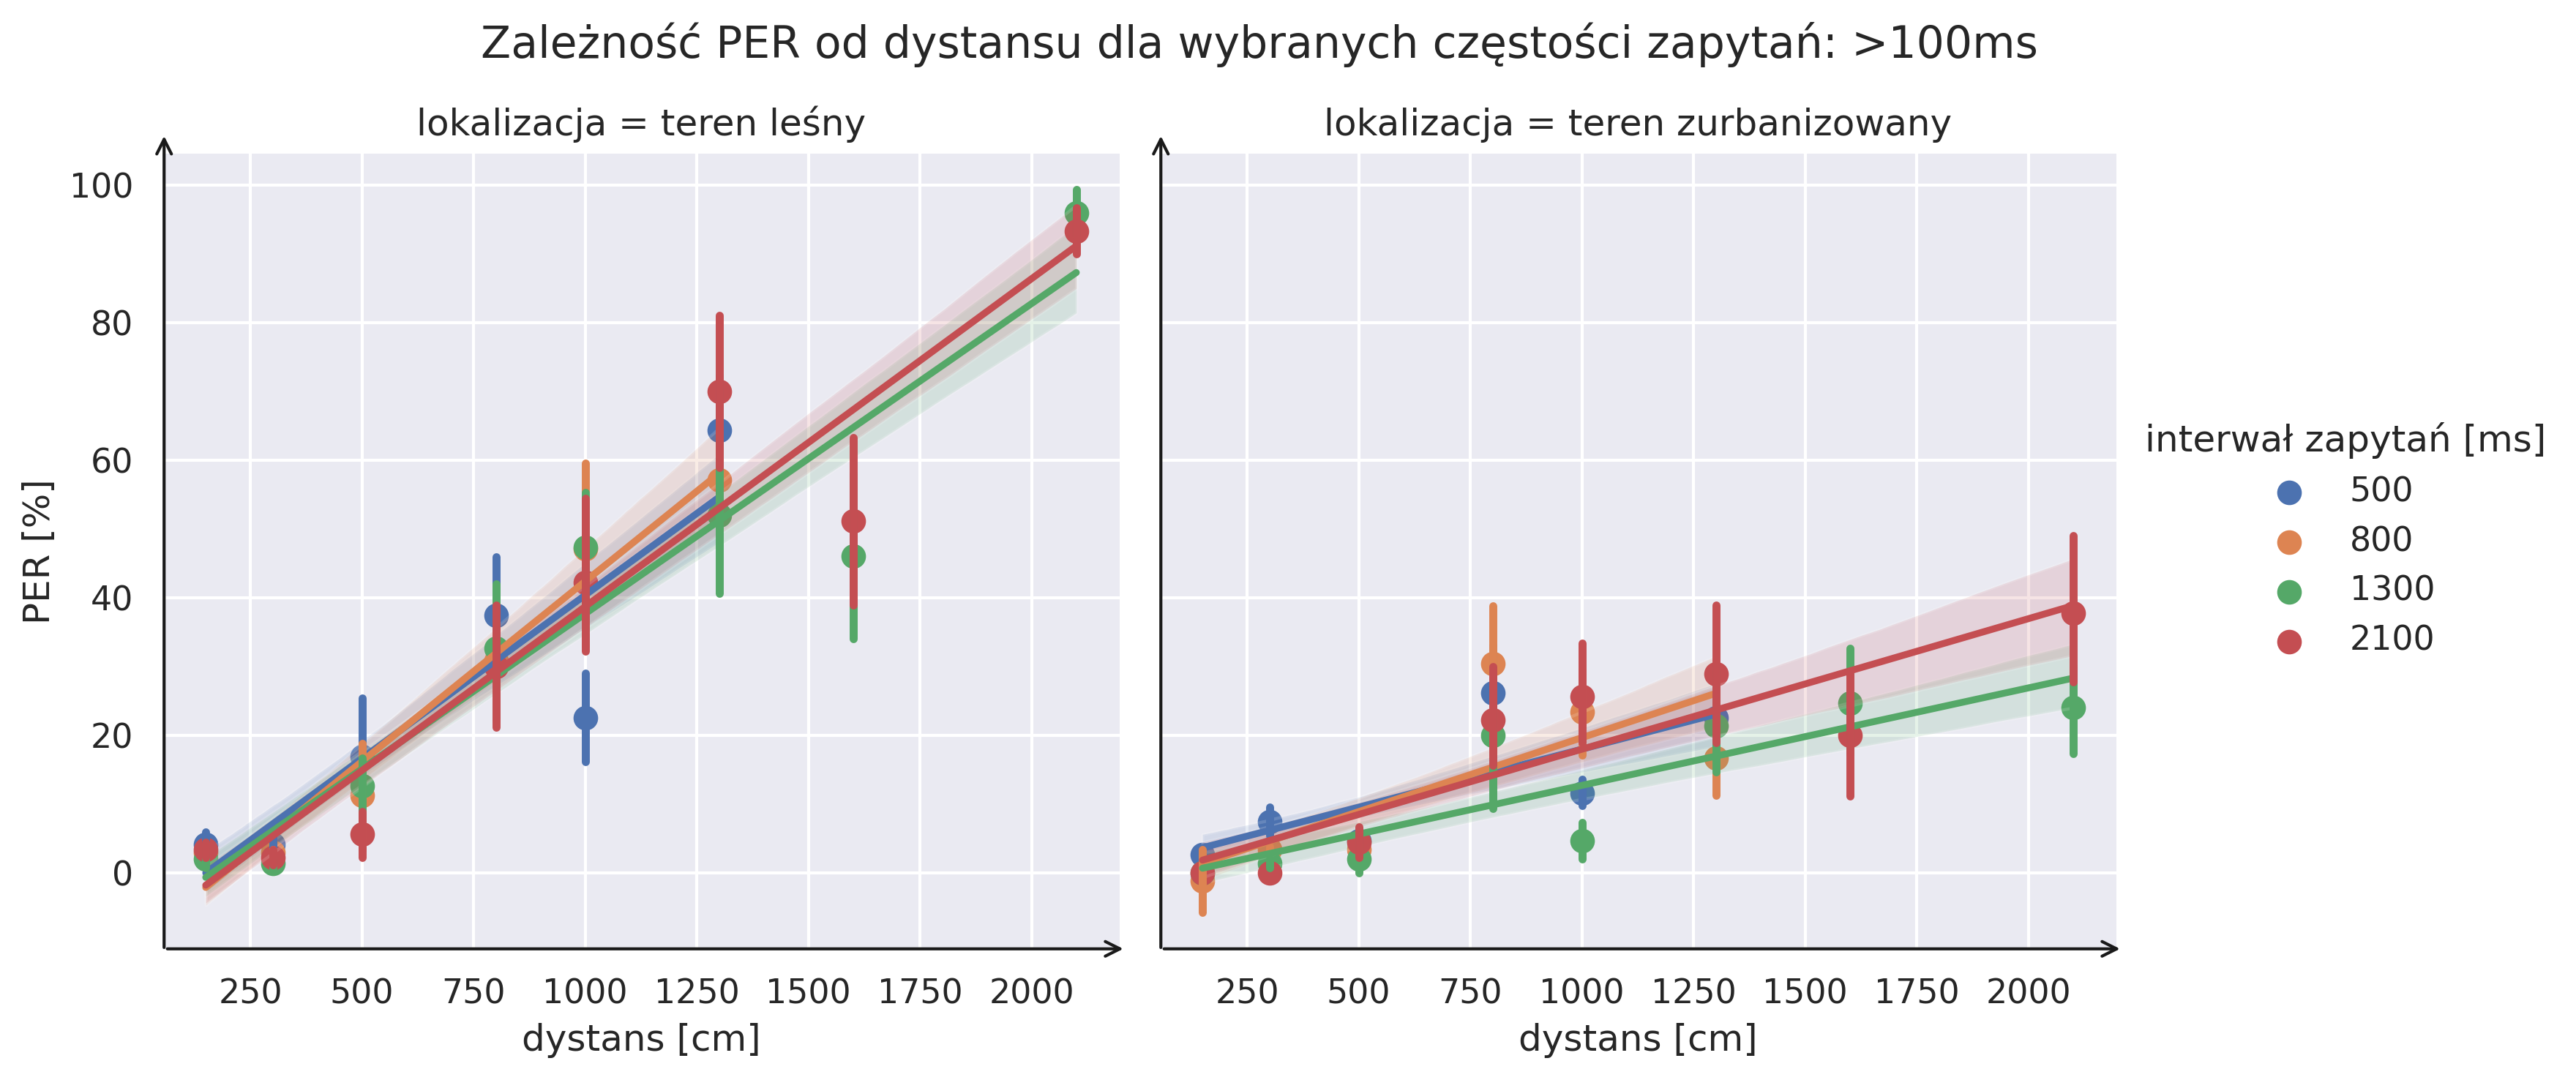
\includegraphics[width=0.99\linewidth]{per_to_distance_over_100ms_different_envs_different_ping_interval.png} 
	\caption{Zależność \gls{PER} od dystansu dla zapytań o częstości >100ms w wybranych środowiskach}
	\label{rys:per_to_distance_over_100ms_different_envs_different_ping_interval}
\end{figure}

Zależność pomiędzy PER a częstością odpytywań została zbadana wykorzystując narzędzia statystyczne. Traktując model
liniowy, jak sugerują zaprezentowane wykresy, tworzonych zgodnie z~metodą najmniejszych kwadratów wylicza się 
współczynnik determinacji dla następujących zmiennych niezależnych: dystans oraz PER. W~kolejnym kroku uwzględnia
się fakt wykorzystywania korelacji wielu zmiennych, dostosowując odpowiednio wartość.


\begin{table}[!ht]
\centering
	\begin{tabular}{p{4.5cm}|r|r}
	Środowisko              & $R^2$             & $R^2_{dostosowany}$\\\hline
	Teren leśny             & 0.04958           & 0.04272\\\hline
	Teren zurbanizowany     & 0.04887           & 0.04200\\\hline
	\end{tabular}
\caption{\label{tab:corr_between_ping_intervals}Współczynnik determinacji dla zależności interwału zapytań od dystansu i~PER w~wybranych środowiskach}
\end{table}

Ostatecznie, otrzymany współczynnik determinacji przyjmujący wartość $R^2=0,04-0,05$.  Istnieje 4\%-owy wpływ
interwału zapytań o częstościach większych niż 100 milisekund na ostateczny rezultat PER. Pozwala to
wykluczyć ten czynnik wykluczyć z dalszych rozważań uznając go za marginalny.

%%%%%%%%%%%%%%%%%%%%%%%%%%%%%%%%%%%%%%%%%%%%%%%%%%%%%%%%%%%%%%%%%%%%%%%%%%%%%%%%
%% SUBSECTION: Zależność \gls{PER} względem odległości między węzłami
%%%%%%%%%%%%%%%%%%%%%%%%%%%%%%%%%%%%%%%%%%%%%%%%%%%%%%%%%%%%%%%%%%%%%%%%%%%%%%%%
\subsection{Zależność PER względem odległości między węzłami}

Ustaliwszy brak (pomijalnie mały) wpływu częstości zapytań (dla częstości wartości >100ms), praca podejmuje dalszą prezentację
danych pod postacią zależności odległości na PER.

Rysunek~\ref{rys:per_to_distance_over_100ms} przedstawia zebrane dane zestawiając odległość i~ilość węzłów składających
się na sieć Mesh. Na początkowych dystansach PER ma wartość bliską bądź równą zeru. Wraz ze wzrostem odległości pomiędzy
węzłami, badany współczynnik rośnie, co jest zgodne z oczekiwaniami. Na dystansie 16m obserwuje się przełamanie
linii aproksymacji. Dodatkowy węzeł środkowy znacząco i pozytywnie wpływa na PER przy kolejnych odległościach
umożliwiając przekazywanie informacji w~sieci. PER w najdalszym punkcie pomiarowym osiąga wartości od ok.~60\% do 70\%.
Należy jednak mieć na uwadze, iż zestawienie nie rozróżnia środowiska w którym następowało zliczanie pakietów.


\begin{figure}[!htb]
	\centering 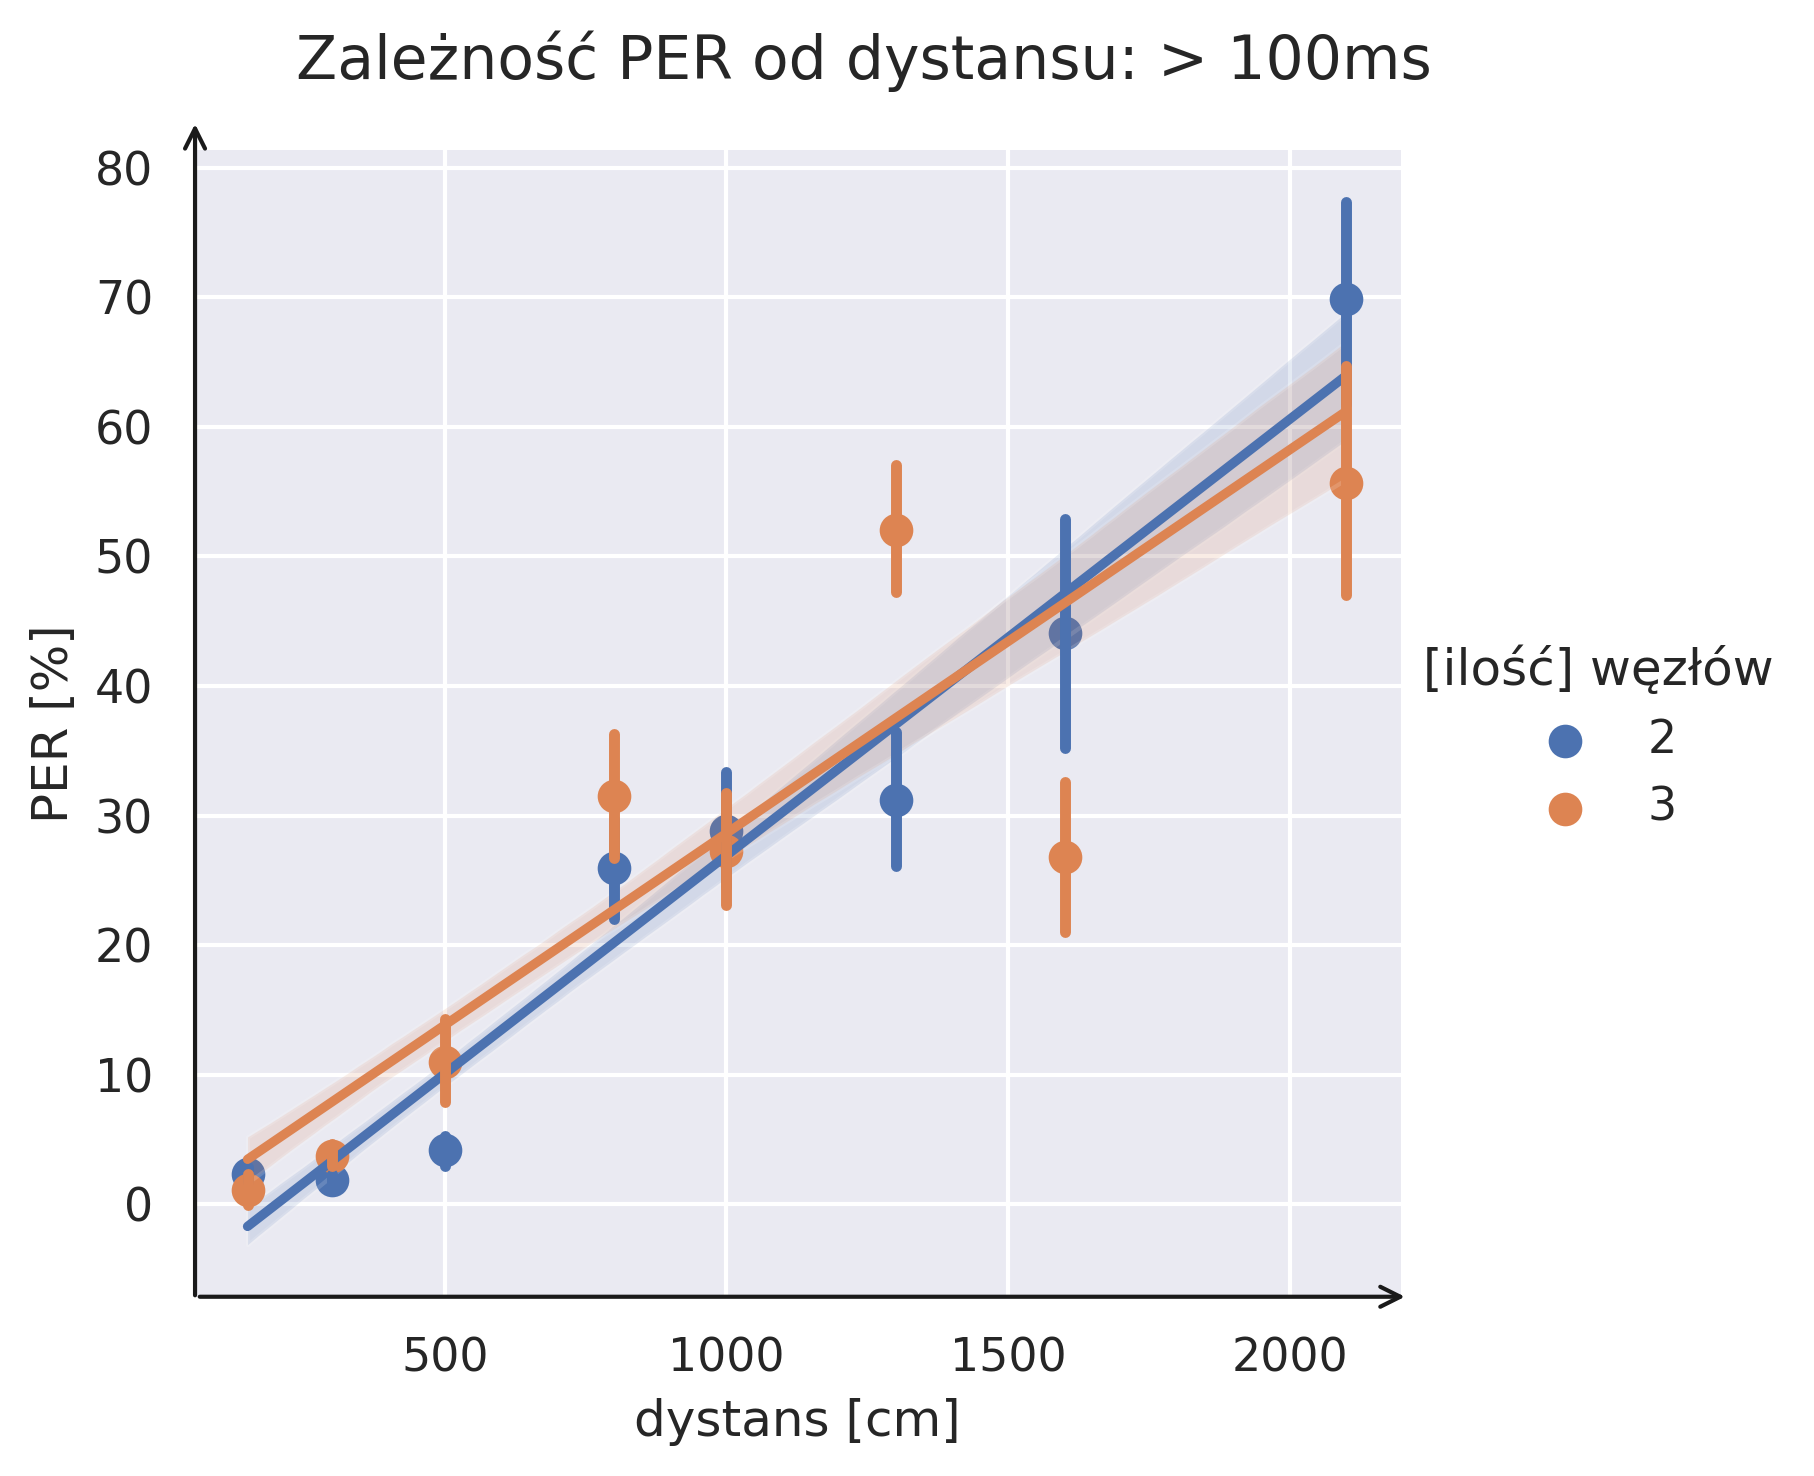
\includegraphics[width=0.618\linewidth]{per_to_distance_over_100ms.png}
	\caption{Zależność \gls{PER} od dystansu dla zapytań o częstości >100ms dla różnej liczby węzłów}
	\label{rys:per_to_distance_over_100ms}
\end{figure}

Rysunek~\ref{rys:per_to_distance_over_100ms_different_envs} uwzględnia wpływ środowiska na PER. Wykres zdecydowanie
wskazuje na różnicę pomiędzy terenem zurbanizowanym a terenem leśnym. Na początkowych dystansach PER jest zbliżone
niezależnie od odległości międzywęzłowych. Znaczące różnice w pomiarach, a dzięki temu również względem linii aproksymacyjnej,
występują już na dystansie 5m. PER w przypadku miejskim jest bliskie zera, gdzie analogiczne pomiary w środowisku
leśnym sugerują piętnastoprocentowy poziom zgubionych pakietów. Wraz ze wzrostem dystansu, wartość PER wzrasta.
Niemniej jednak nachylenie linii wskazuje na zdecydowanie wolniejsze narastanie utraty danych podczas transmisji
bezprzewodowej dla przypadku miejskiego. Na maksymalnym dystansie międzywęzłowym wynoszącym 21m, PER
przybiera wartość ok. 30\%. W analogicznym przypadku dla środowiska leśnego następuje niemal całkowita utrata
transmisji.

\begin{figure}[!htb]
	\centering 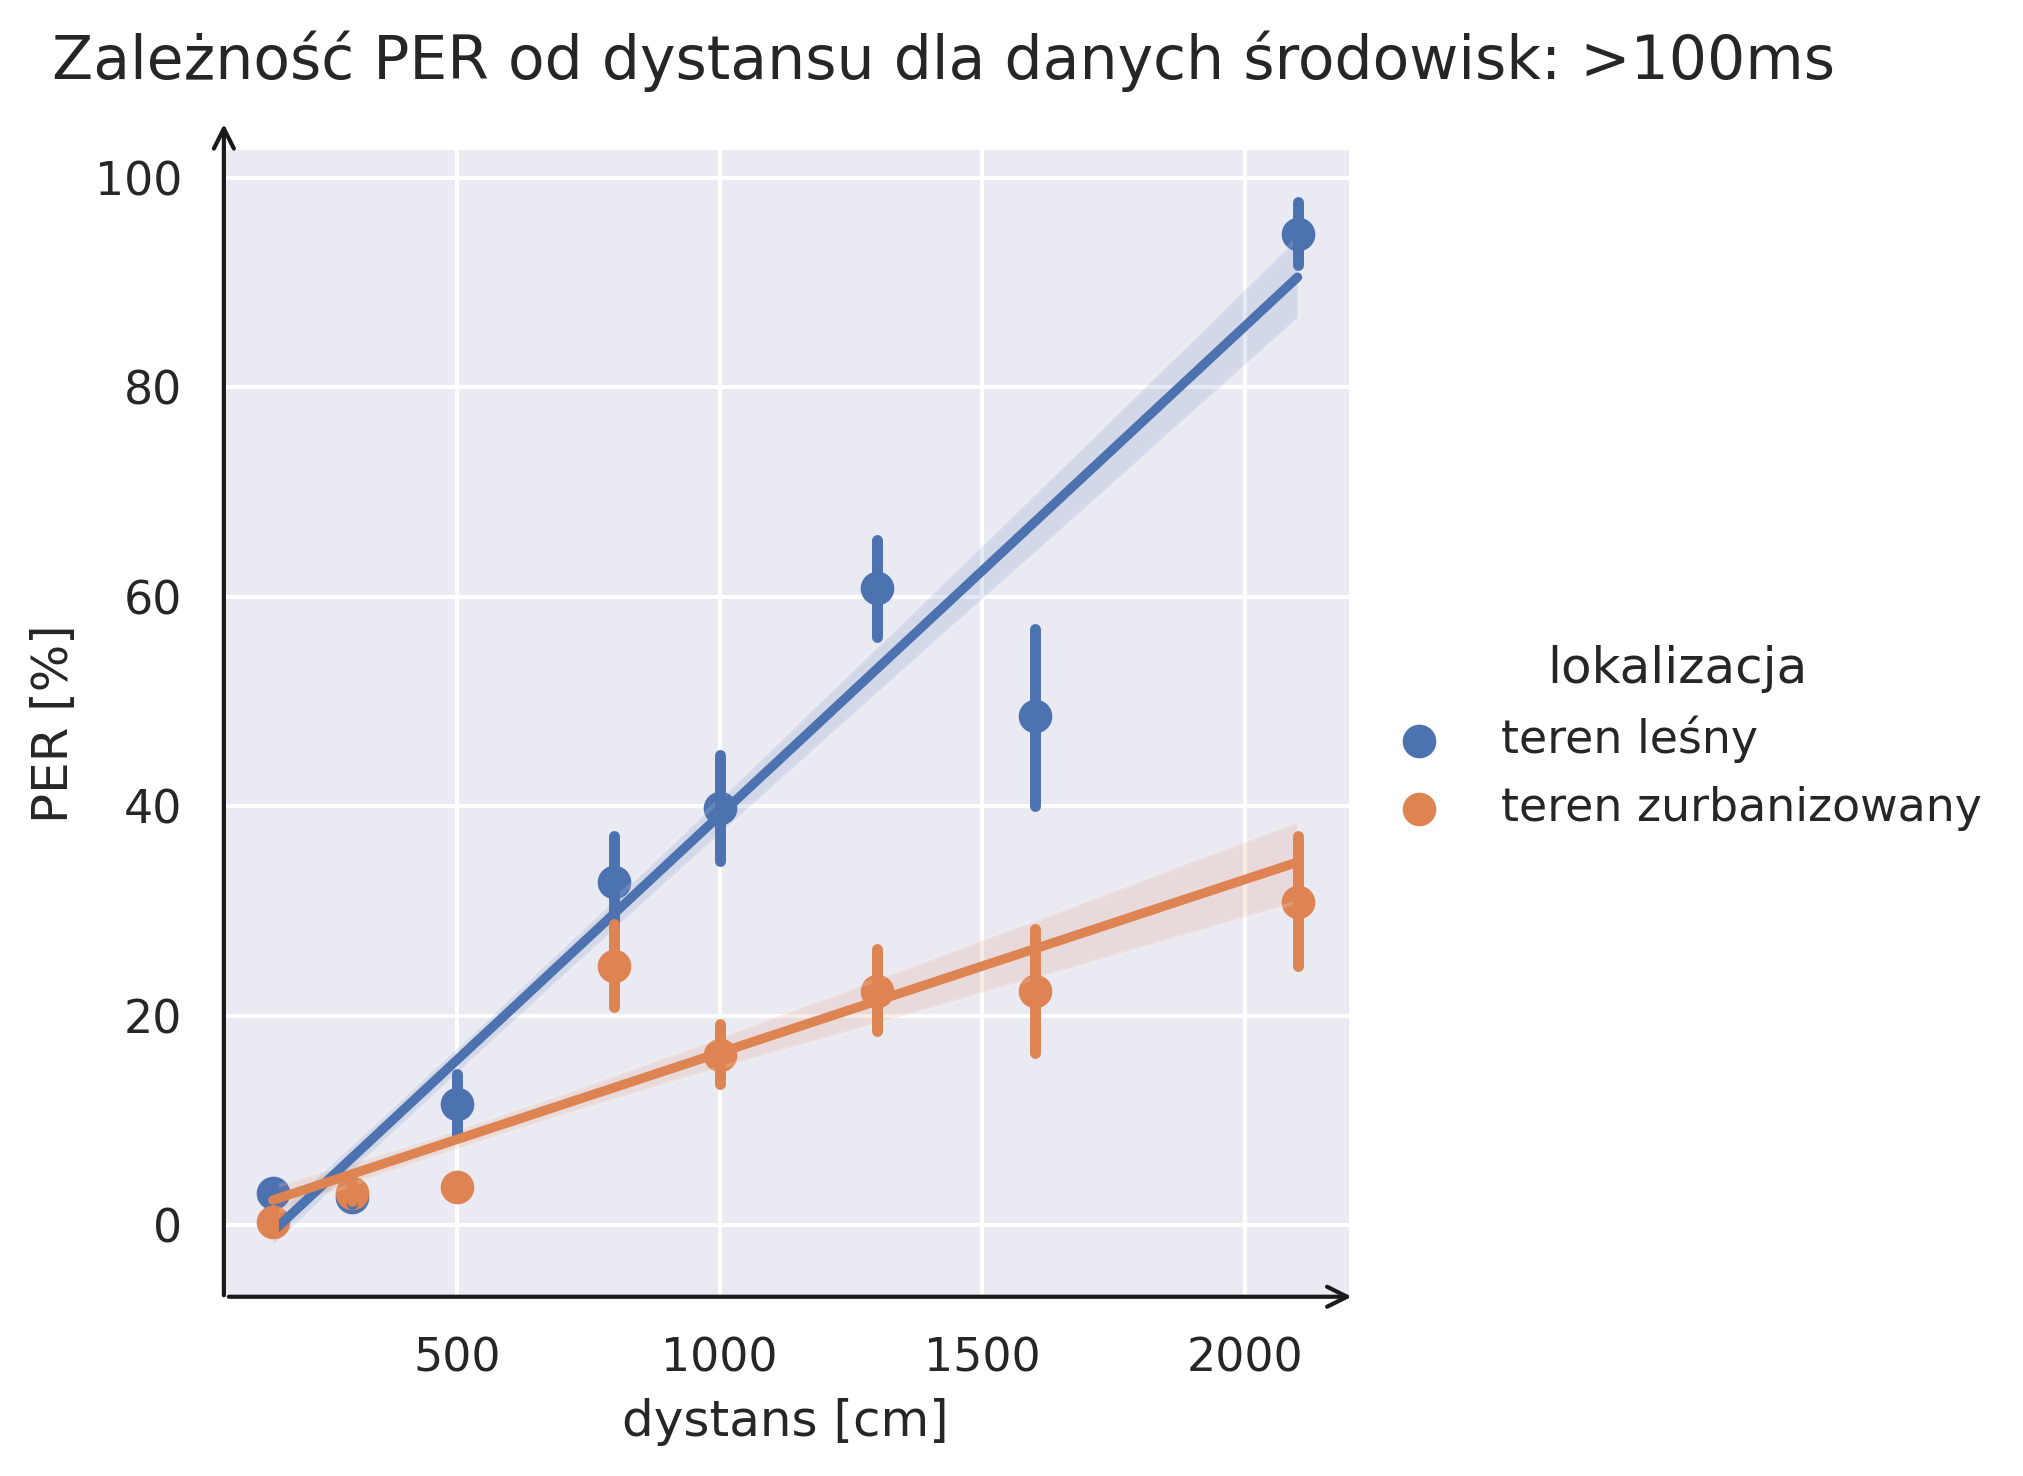
\includegraphics[width=0.618\linewidth]{per_to_distance_over_100ms_different_envs.png} 
	\caption{Zależność \gls{PER} od dystansu dla zapytań o częstości >100ms w wybranych środowiskach bez rozróżnienia na liczbę węzłów}
	\label{rys:per_to_distance_over_100ms_different_envs}
\end{figure}

% w sumie, ta korelacja praktycznie nic wartościowego nie przedstawia. Wymyślić inny współczynnik albo w ogóle wyrzucić tą tabelkę
\begin{table}[!ht]
\centering
	\begin{tabular}{p{4.5cm}|r}
	Środowisko              & $r$             \\\hline
	Teren leśny             & 0.62262         \\\hline
	Teren zurbanizowany     & 0.23582         \\\hline
	\end{tabular}
\caption{\label{tab:corr_between_per_and_env}Współczynnik korelacji Pearsona dla zależności PER od odległości międzywęzłowej dla zadanych środowisk}
\end{table}

Ostatnia prezentowana zależność ukazana jest na Rysunku~\ref{rys:per_to_distance_over_100ms_different_envs_and_nodes}.
Przedstawia on zależność PER od dystansu dla wybranych środowisk i liczby węzłów. Uwidaczniają się wyżej wymienione
cechy transmisji opisane w poprzednich akapitach.

Dla przypadku dwóch węzłów, PER jest bliskie zeru na początkowych dystansach do 5m niezależnie od środowiska. W odległości 8m
od stacji bazowej obserwuje się miejscową anomalię polegającą na blisko 40\%-ej utraty pakietów dla terenu zurbanizowanego.
Zarówno jak w~poprzednich jak i~kilku następujących po sobie punktach pomiarowych, PER nie przybiera takich wartości. Anomalia może
być wytłumaczona cechami środowiska - np. węzeł dalszy ułożony został w zagłębieniu, co utrudniło odbiór propagowanej fali
radiowej. W pozostałych punktach pomiarowych w terenie zurbanizowanym obserwuje się spadek wartości PER wraz ze zwiększanym dystansem,
co znów sugeruje wpływ ukształtowania terenu. Utrata pakietów wynosząca niewiele powyżej 40\% zaobserwowana jest na odległości
21m. Jest to o tyle zaskakujące, o tyle dla analogicznego dystansu pomiarowego w terenie leśnym PER wynosi niemal 100\%.

Charakterystyka transmisji dla badanego przypadku trzech węzłów przybiera podobną postać. Wartości PER w terenie zurbanizowanym są zbliżone
w początkowych dystansach pomiarowych. Dystans 8m (węzeł dalszy na odległości 16m) wskazuje na analogiczną anomalię jak w~opisywanym
przypadku dwóch węzłów. Obserwuje się maksimum lokalne PER poniżej 20\% w otoczeniu najbliższych punktów pomiarowych. Kolejne pomiary
wskazują na stały przyrost PER względem równoodległych węzłów. Utrata pakietów na maksymalnym całkowitym dystansie 42m wynosi ok. 20\%.

Transmisja danych w środowisku leśnym charakteryzuje się większym przyrostem PER względem odległości w~porównaniu do warunków miejskich.
Przypadek dwuwęzłowej sieci wskazuje zbliżone wartości utraty pakietów na odległości do 5m włącznie. Na każdym kolejnym dystansie
pomiarowym PER wzrasta zbliżając się do 100\% w miejscu oddalonym o 21m od węzła bliższego. Oznacza to niemal całkowitą utratę łączności.
Charakterystyka dla sieci zbudowanej z trzech węzłów jest analogiczna. Wyjątkiem jest zbiór pomiarów zebranych na dystansie pomiędzy węzłami
wynoszącym 16m. PER w tym przypadku spada do ok. 20\%. Jest to o tyle niespodziewane iż, poprzedzające i~następujące pomiary i~wynikłe
w~konsekwencji PER są blisko 4-krotnie wyższe. Taką konsekwencje należy przypisać ukształtowaniu terenu aniżeli nieznanej właściwości
transmisji radiowej.

\begin{figure}[!htb]
	\centering 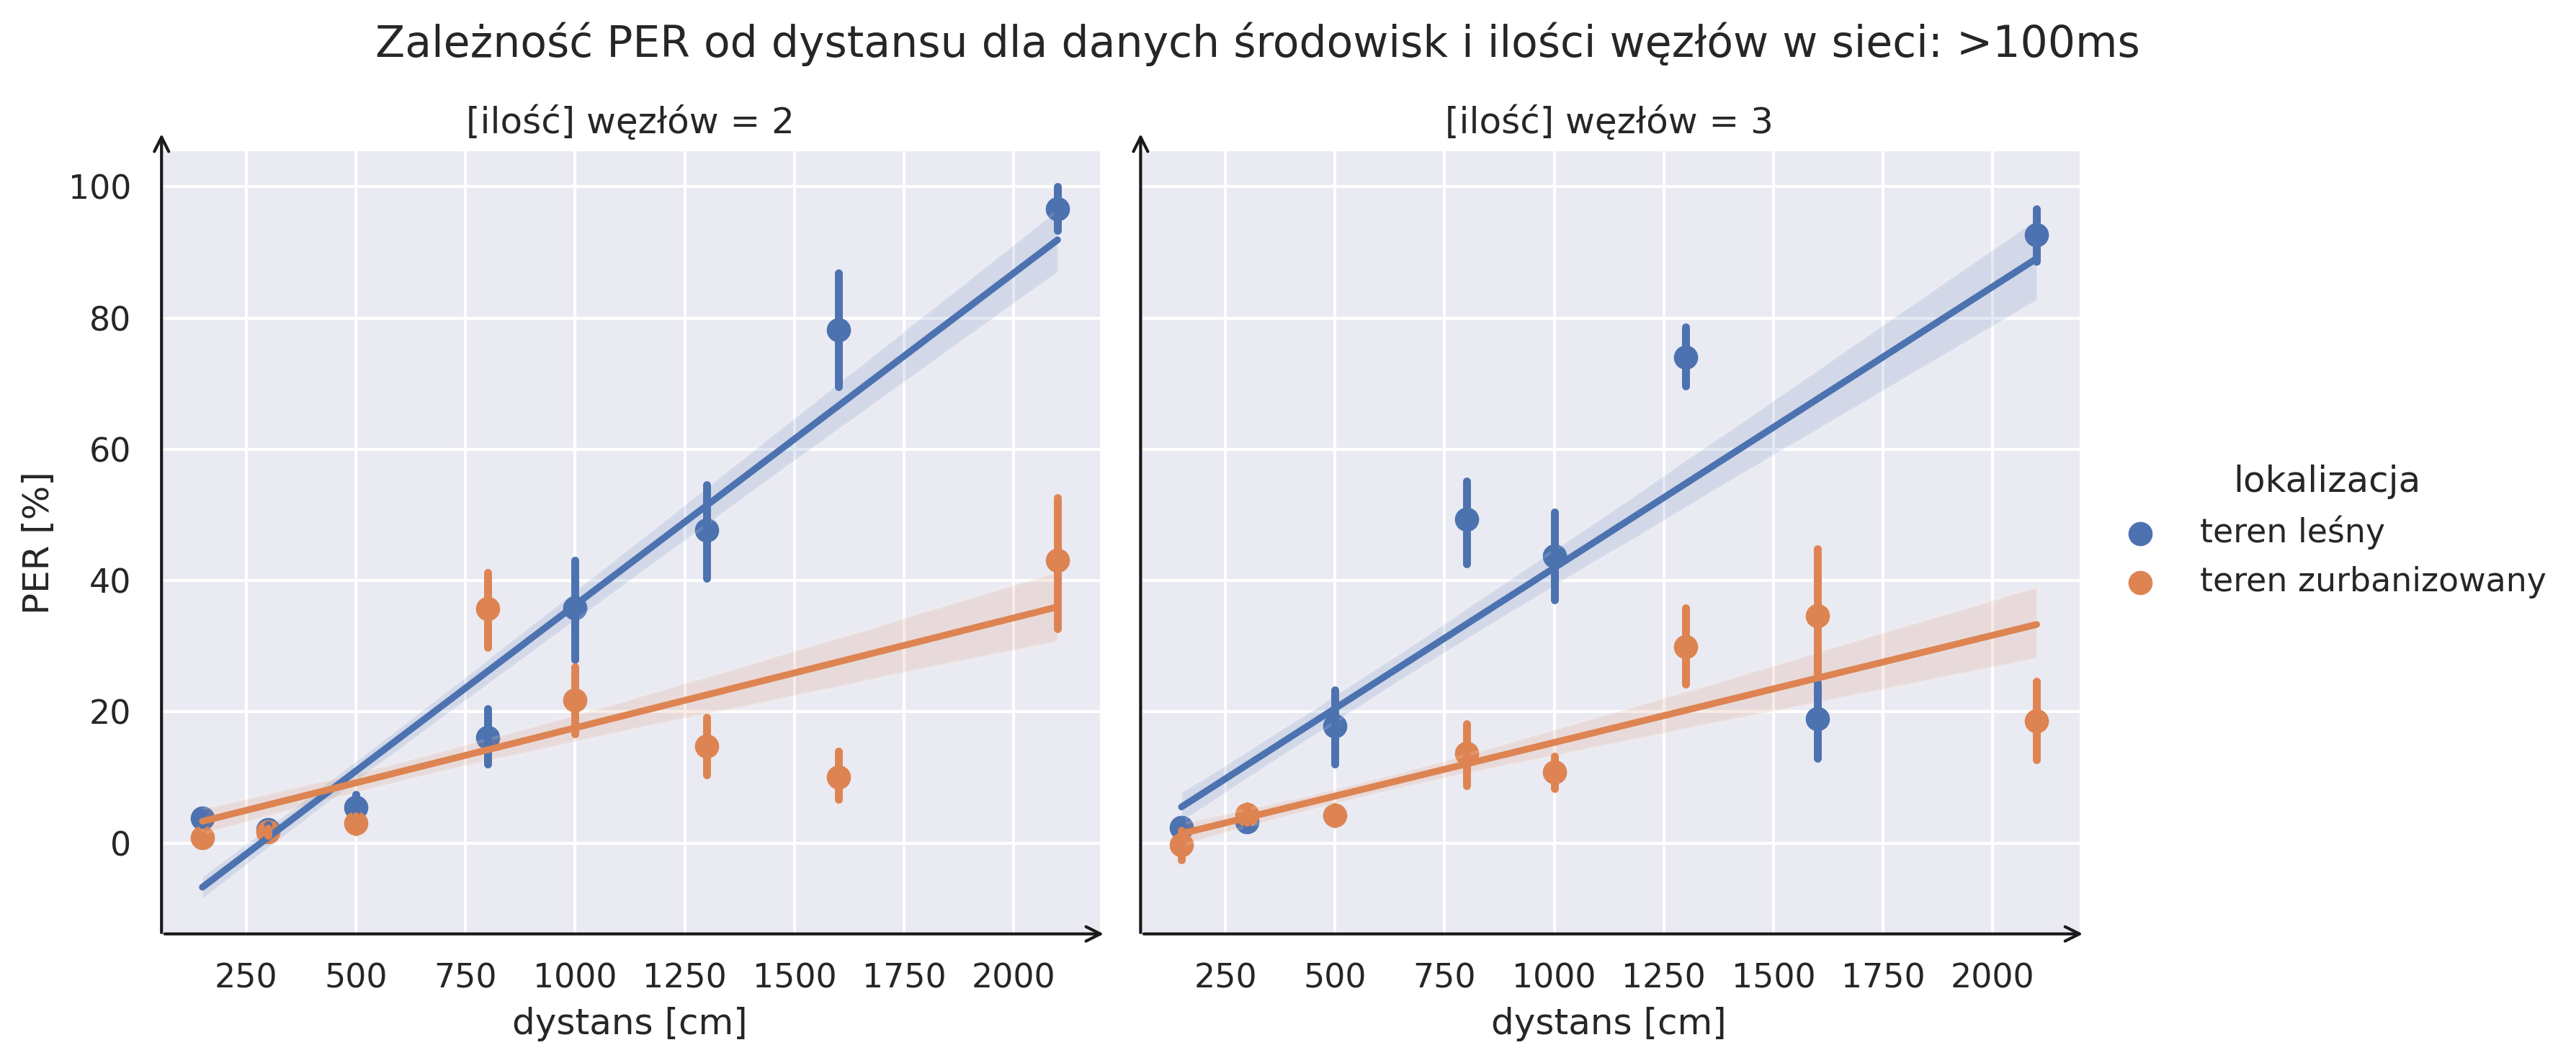
\includegraphics[width=0.99\linewidth]{per_to_distance_over_100ms_different_envs_and_nodes.png}
	\caption{Zależność \gls{PER} od dystansu dla zapytań o częstości >100ms w wybranych środowiskach i liczbę badanych węzłów}
	\label{rys:per_to_distance_over_100ms_different_envs_and_nodes}
\end{figure}

% opisać brak jasnych punktów przełamania. Nieznany moment wpływu dodatkowego węzła wynikający z braku warunków laboratoryjnych
% w których strefa Fresnela byłaby bardziej przewidywalna.

Przedstawione dane prezentują wpływ dystansu na PER w różnych środowiskach. Określona kategoria badanych środowisk nie jest jedynym
parametrem charakteryzującym przeprowadzone badania. Dużą odpowiedzialność w~ostatecznych zebranych wartościach należy położyć
na czynniki takie jak ukształtowanie terenu i pogoda. Pomimo organoleptycznego doboru terenu o możliwie nieurozmaiconej charakterystyce,
badane węzły mogły zostać ułożone w lokalnym zagłębieniu wynikłym z~gleby bądź nawet zagęszczeniu trawy w danym miejscu. Różnica
w~wilgotności również mogła mieć znaczenie w~zebranych danych. Niepewności te są konsekwencją metodologii przeprowadzonych
badań w warunkach nielaboratoryjnych (terenowych). Czynniki te, nie będące częścią formalnie zebranych danych, najprawdopodobniej
miały wpływ na ilość odebranych pakietów. Ukształtowanie terenu jak i wilgotność mają bezpośredni wpływ jakość transmisji stanowiąc
przeszkody dla strefy propagacji sygnału radiowego (strefy Fresnela).

